\documentclass[a4paper,12pt]{article}
\usepackage{amsmath, amssymb}
\usepackage{xcolor}
\usepackage[most]{tcolorbox}
\usepackage{geometry}
\usepackage{tkz-tab}
\graphicspath{ {../Images/} }

\geometry{left=1.5cm, right=1.5cm, top=1.5cm, bottom=1.5cm}

\title{Exercices de Polynômes de Degré 2 - Niveau Première}
\author{}
\date{}

\definecolor{PurpleEx}{HTML}{5d478b}
\definecolor{GrayEx}{HTML}{f2f2f2}
\definecolor{GrayBG}{HTML}{d9d9d9}
\definecolor{BlackSav}{HTML}{000000}

% Style de boîte pour les exercices
\tcbset{
    colframe=purple!70,
    colback=white,
    coltitle=black,
    fonttitle=\bfseries,
    sharp corners,
    boxrule=0.5mm,
    colbacktitle=purple!20!white,
    center title,
    boxsep=4pt,
}

\newtcbtheorem
  []% init options
  {exercice}% name
  {Exercice}% title
  {%
    colback=GrayEx,
    colframe=PurpleEx,
    fonttitle=\bfseries,
  }% options
  {ex}% prefix

% Style de boîte pour les solutions
\newtcolorbox{solutionbox}[1][]{
    colframe=green!70,
    colback=white,
    coltitle=black,
    fonttitle=\bfseries,
    sharp corners,
    boxrule=0.5mm,
    colbacktitle=green!20!white,
    title=Solution,
    boxsep=4pt,
    breakable,
    #1
}

\begin{document}

% % Exercice 1
% \begin{tcolorbox}[title=Exercice 1 * {Calculer}]
% Calculer le discriminant de chaque polynôme ci-dessous.
% \begin{enumerate}
%     \item $3x^2 + 2x + 1$
%     \item $2x^2 - 2x - 4$
%     \item $-3x^2 + 2x - 5$
%     \item $x^2 + x + 1$
%     \item $x^2 - 7$
%     \item $x - x^2 + 3$
%     \item $7x - 3 + x^2$
%     \item $1 - 3x^2$
% \end{enumerate}
% \end{tcolorbox}
% 
% \begin{solutionbox}
% Pour chaque polynôme de la forme $ax^2 + bx + c$, le discriminant est $\Delta = b^2 - 4ac$.
% 
% \begin{enumerate}
%     \item $3x^2 + 2x + 1$
% 
%     Coefficients : $a = 3$, $b = 2$, $c = 1$
% 
%     Calcul du discriminant :
% \[
%     \Delta = b^2 - 4ac = (2)^2 - 4 \times 3 \times 1 = 4 - 12 = -8
% \]
% 
%     \item $2x^2 - 2x - 4$
% 
%     Coefficients : $a = 2$, $b = -2$, $c = -4$
% 
%     Calcul du discriminant :
% \[
%     \Delta = (-2)^2 - 4 \times 2 \times (-4) = 4 + 32 = 36
% \]
% 
%     \item $-3x^2 + 2x - 5$
% 
%     Coefficients : $a = -3$, $b = 2$, $c = -5$
% 
%     Calcul du discriminant :
% \[
%     \Delta = (2)^2 - 4 \times (-3) \times (-5) = 4 - 60 = -56
% \]
% 
%     \item $x^2 + x + 1$
% 
%     Coefficients : $a = 1$, $b = 1$, $c = 1$
% 
%     Calcul du discriminant :
% \[
%     \Delta = (1)^2 - 4 \times 1 \times 1 = 1 - 4 = -3
% \]
% 
%     \item $x^2 - 7$
% 
%     Coefficients : $a = 1$, $b = 0$, $c = -7$
% 
%     Calcul du discriminant :
% \[
%     \Delta = (0)^2 - 4 \times 1 \times (-7) = 0 + 28 = 28
% \]
% 
%     \item $x - x^2 + 3$
% 
%     Réécrivons le polynôme sous la forme standard :
% \[
%     -x^2 + x + 3
% \]
%     Coefficients : $a = -1$, $b = 1$, $c = 3$
% 
%     Calcul du discriminant :
% \[
%     \Delta = (1)^2 - 4 \times (-1) \times 3 = 1 + 12 = 13
% \]
% 
%     \item $7x - 3 + x^2$
% 
%     Réécrivons le polynôme :
% \[
%     x^2 + 7x - 3
% \]
%     Coefficients : $a = 1$, $b = 7$, $c = -3$
% 
%     Calcul du discriminant :
% \[
%     \Delta = (7)^2 - 4 \times 1 \times (-3) = 49 + 12 = 61
% \]
% 
%     \item $1 - 3x^2$
% 
%     Réécrivons le polynôme :
% \[
%     -3x^2 + 1
% \]
%     Coefficients : $a = -3$, $b = 0$, $c = 1$
% 
%     Calcul du discriminant :
% \[
%     \Delta = (0)^2 - 4 \times (-3) \times 1 = 0 + 12 = 12
% \]
% \end{enumerate}
% \end{solutionbox}
% 
% % Exercice 2
% \begin{tcolorbox}[title=Exercice 2 * {Calculer}]
% Déterminer la forme factorisée, lorsqu’elle existe, des polynômes suivants.
% \begin{enumerate}
%     \item $x^2 + 3x - 4$
%     \item $2x^2 - 4x - 12$
%     \item $-3x^2 + x - 5$
%     \item $x^2 + x + 1$
%     \item $x^2 - 2x + 1$
%     \item $x - 4x^2 + 2$
% \end{enumerate}
% \end{tcolorbox}
% 
% \begin{solutionbox}
% Pour factoriser un polynôme de degré 2, on calcule son discriminant $\Delta$.
% 
% \begin{enumerate}
%     \item $x^2 + 3x - 4$
% 
%     $\Delta = 3^2 - 4 \times 1 \times (-4) = 9 + 16 = 25$
% 
%     Les racines sont :
% \[
%     x = \dfrac{-b \pm \sqrt{\Delta}}{2a} = \dfrac{-3 \pm 5}{2}
% \]
%     Donc :
% \[
%     x_1 = \dfrac{-3 + 5}{2} = 1 \quad \text{et} \quad x_2 = \dfrac{-3 - 5}{2} = -4
% \]
% 
%     La forme factorisée est :
% \[
%     x^2 + 3x - 4 = (x - x_1)(x - x_2) = (x - 1)(x + 4)
% \]
% 
%     \item $2x^2 - 4x - 12$
% 
%     $\Delta = (-4)^2 - 4 \times 2 \times (-12) = 16 + 96 = 112$
% 
%     Les racines sont :
% \[
%     x = \dfrac{4 \pm \sqrt{112}}{4} = \dfrac{4 \pm 4 \sqrt{7}}{4} = \dfrac{4(1 \pm \sqrt{7})}{4} = 1 \pm \sqrt{7}
% \]
% 
%     La forme factorisée est :
% \[
%     2x^2 - 4x - 12 = 2 \left( x - \left( 1 + \sqrt{7} \right) \right) \left( x - \left( 1 - \sqrt{7} \right) \right)
% \]
% 
%     \item $-3x^2 + x - 5$
% 
%     $\Delta = 1^2 - 4 \times (-3) \times (-5) = 1 - 60 = -59$
% 
%     Comme $\Delta < 0$, le polynôme n'est pas factorisable dans $\mathbb{R}$.
% 
%     \item $x^2 + x + 1$
% 
%     $\Delta = 1^2 - 4 \times 1 \times 1 = 1 - 4 = -3$
% 
%     Comme $\Delta < 0$, le polynôme n'est pas factorisable dans $\mathbb{R}$.
% 
%     \item $x^2 - 2x + 1$
% 
%     $\Delta = (-2)^2 - 4 \times 1 \times 1 = 4 - 4 = 0$
% 
%     Une racine double :
% \[
%     x = \dfrac{2}{2} = 1
% \]
% 
%     La forme factorisée est :
% \[
%     x^2 - 2x + 1 = (x - 1)^2
% \]
% 
%     \item $x - 4x^2 + 2$
% 
%     Réécrivons le polynôme :
% \[
%     -4x^2 + x + 2
% \]
% 
%     Coefficients : $a = -4$, $b = 1$, $c = 2$
% 
%     $\Delta = 1^2 - 4 \times (-4) \times 2 = 1 + 32 = 33$
% 
%     Racines :
% \[
%     x = \dfrac{-1 \pm \sqrt{33}}{-8} = \dfrac{-1 \pm \sqrt{33}}{-8}
% \]
% 
%     La forme factorisée est :
% \[
%     -4x^2 + x + 2 = -4 \left( x - x_1 \right) \left( x - x_2 \right)
% \]
% 
%     avec $x_1 = \dfrac{-1 + \sqrt{33}}{-8}$ et $x_2 = \dfrac{-1 - \sqrt{33}}{-8}$.
% 
% \end{enumerate}
% \end{solutionbox}
% 
% % Exercice 3
% \begin{tcolorbox}[title=Exercice 3 * {Calculer}]
% Résoudre dans $ \mathbb{R} $ les équations suivantes.
% \begin{enumerate}
%     \item $x^2 + x - 4 = 0$
%     \item $3x^2 - x - 6 = 0$
%     \item $x^2 - 10x + 25 = 0$
%     \item $x^2 - 3x + 3 = 0$
%     \item $x^2 - 1 = 0$
%     \item $x - 4x^2 + 7 = 0$
% \end{enumerate}
% \end{tcolorbox}
% 
% \begin{solutionbox}
% Résolvons chaque équation en calculant le discriminant.
% 
% \begin{enumerate}
%     \item $x^2 + x - 4 = 0$
% 
%     $\Delta = 1^2 - 4 \times 1 \times (-4) = 1 + 16 = 17$
% 
%     Racines :
% \[
%     x = \dfrac{-1 \pm \sqrt{17}}{2}
% \]
% 
%     \item $3x^2 - x - 6 = 0$
% 
%     $\Delta = (-1)^2 - 4 \times 3 \times (-6) = 1 + 72 = 73$
% 
%     Racines :
% \[
%     x = \dfrac{1 \pm \sqrt{73}}{6}
% \]
% 
%     \item $x^2 - 10x + 25 = 0$
% 
%     $\Delta = (-10)^2 - 4 \times 1 \times 25 = 100 - 100 = 0$
% 
%     Racine double :
% \[
%     x = \dfrac{10}{2} = 5
% \]
% 
%     \item $x^2 - 3x + 3 = 0$
% 
%     $\Delta = (-3)^2 - 4 \times 1 \times 3 = 9 - 12 = -3$
% 
%     Pas de solution réelle.
% 
%     \item $x^2 - 1 = 0$
% 
%     $\Delta = 0^2 - 4 \times 1 \times (-1) = 0 + 4 = 4$
% 
%     Racines :
% \[
%     x = \dfrac{0 \pm 2}{2} = \pm 1
% \]
% 
%     \item $x - 4x^2 + 7 = 0$
% 
%     Réécrivons l'équation :
% \[
%     -4x^2 + x + 7 = 0
% \]
% 
%     $\Delta = 1^2 - 4 \times (-4) \times 7 = 1 + 112 = 113$
% 
%     Racines :
% \[
%     x = \dfrac{-1 \pm \sqrt{113}}{-8}
% \]
% \end{enumerate}
% \end{solutionbox}
% 
% % Exercice 4
% \begin{tcolorbox}[title=Exercice 4 * {Calculer}]
% Déterminer les racines des polynômes suivants.
% \begin{enumerate}
%     \item $x^2 - x - 1$
%     \item $x^2 - x$
%     \item $-5x^2 + 7x + 12$
%     \item $-3x - x^2 + 4$
%     \item $3x^2 - 6x + 3$
%     \item $-x + x^2 + 7$
% \end{enumerate}
% \end{tcolorbox}
% 
% \begin{solutionbox}
% \begin{enumerate}
%     \item $x^2 - x - 1$
% 
%     $\Delta = (-1)^2 - 4 \times 1 \times (-1) = 1 + 4 = 5$
% 
%     Racines :
% \[
%     x = \dfrac{1 \pm \sqrt{5}}{2}
% \]
% 
%     \item $x^2 - x$
% 
%     Mise en évidence :
% \[
%     x(x - 1) = 0
% \]
%     Les racines sont $x = 0$ et $x = 1$.
% 
%     \item $-5x^2 + 7x + 12$
% 
%     $\Delta = 7^2 - 4 \times (-5) \times 12 = 49 + 240 = 289$
% 
%     Racines :
% \[
%     x = \dfrac{-7 \pm 17}{-10}
% \]
% 
%     Calculons :
% \[
%     x_1 = \dfrac{-7 + 17}{-10} = \dfrac{10}{-10} = -1
% \]
% \[
%     x_2 = \dfrac{-7 - 17}{-10} = \dfrac{-24}{-10} = \dfrac{12}{5}
% \]
% 
%     \item $-3x - x^2 + 4$
% 
%     Réécrivons :
% \[
%     -x^2 - 3x + 4 = 0
% \]
%     Puis multiplions par $-1$ :
% \[
%     x^2 + 3x - 4 = 0
% \]
% 
%     $\Delta = 3^2 - 4 \times 1 \times (-4) = 9 + 16 = 25$
% 
%     Racines :
% \[
%     x = \dfrac{-3 \pm 5}{2}
% \]
% 
%     Donc :
% \[
%     x_1 = \dfrac{-3 + 5}{2} = 1 \quad \text{et} \quad x_2 = \dfrac{-3 - 5}{2} = -4
% \]
% 
%     \item $3x^2 - 6x + 3$
% 
%     $\Delta = (-6)^2 - 4 \times 3 \times 3 = 36 - 36 = 0$
% 
%     Racine double :
% \[
%     x = \dfrac{6}{6} = 1
% \]
% 
%     \item $-x + x^2 + 7$
% 
%     Réécrivons :
% \[
%     x^2 - x + 7 = 0
% \]
% 
%     $\Delta = (-1)^2 - 4 \times 1 \times 7 = 1 - 28 = -27$
% 
%     Pas de racines réelles.
% 
% \end{enumerate}
% \end{solutionbox}
% 
% % Exercice 5
% \begin{tcolorbox}[title=Exercice 5 ** {Calculer, Raisonner}]
% Soit $m \in \mathbb{R}$. On considère l'équation $x^2 - mx + m + 2 = 0$. Pour quelles valeurs de $m$ l'équation admet-elle une unique solution ?
% \end{tcolorbox}
% 
% \begin{solutionbox}
% Une équation du second degré admet une unique solution réelle lorsque son discriminant est nul.
% 
% Calculons le discriminant :
% \[
% \Delta = (-m)^2 - 4 \times 1 \times (m + 2) = m^2 - 4(m + 2)
% \]
% 
% Développons :
% \[
% \Delta = m^2 - 4m - 8
% \]
% 
% Posons $\Delta = 0$ :
% \[
% m^2 - 4m - 8 = 0
% \]
% 
% Résolvons cette équation du second degré en $m$ :
% \[
% \Delta' = (-4)^2 - 4 \times 1 \times (-8) = 16 + 32 = 48
% \]
% 
% Racines :
% \[
% m = \dfrac{4 \pm \sqrt{48}}{2} = \dfrac{4 \pm 4 \sqrt{3}}{2} = 2 \pm 2 \sqrt{3}
% \]
% 
% Ainsi, l'équation admet une unique solution réelle pour :
% \[
% m = 2 + 2 \sqrt{3} \quad \text{ou} \quad m = 2 - 2 \sqrt{3}
% \]
% \end{solutionbox}
% 
% % Exercice 6
% \begin{tcolorbox}[title=Exercice 6 ** {Calculer, Modéliser}]
% Déterminer deux entiers naturels consécutifs dont le produit est égal à 64262.
% \end{tcolorbox}
% 
% \begin{solutionbox}
% Soit $n$ un entier naturel. Les deux entiers consécutifs sont $n$ et $n + 1$.
% 
% Leur produit est :
% \[
% n(n + 1) = 64262
% \]
% 
% Développons :
% \[
% n^2 + n - 64262 = 0
% \]
% 
% Résolvons cette équation du second degré :
% 
% $\Delta = 1^2 - 4 \times 1 \times (-64262) = 1 + 257048 = 257049$
% 
% $\sqrt{\Delta} = \sqrt{257049} = 507$
% 
% Racines :
% \[
% n = \dfrac{-1 \pm 507}{2}
% \]
% 
% Calculons :
% 
% 1) $n = \dfrac{-1 + 507}{2} = \dfrac{506}{2} = 253$
% 
% 2) $n = \dfrac{-1 - 507}{2} = \dfrac{-508}{2} = -254$ (négatif, pas un entier naturel)
% 
% Donc, les deux entiers sont $253$ et $254$.
% 
% \textbf{Réponse :} Les entiers sont $253$ et $254$.
% \end{solutionbox}
% 
% % Exercice 7
% \begin{tcolorbox}[title=Exercice 7 * {Calculer}]
% Les équations suivantes admettent toutes des racines. Dans chaque cas, déterminer le produit et la somme des racines.
% \begin{enumerate}
%     \item $x^2 - x - 2$
%     \item $x^2 - \pi x$
%     \item $-x^2 + 3x + 12$
%     \item $3x + x^2 - 1$
%     \item $\sqrt{17}x^2 + 32x - 1$
%     \item $2x - 3x^2 + 5$
% \end{enumerate}
% \end{tcolorbox}
% 
% \begin{solutionbox}
% Pour un polynôme $ax^2 + bx + c$, la somme des racines est $S = -\dfrac{b}{a}$ et le produit est $P = \dfrac{c}{a}$.
% 
% \begin{enumerate}
%     \item $x^2 - x - 2$
% 
%     Coefficients : $a = 1$, $b = -1$, $c = -2$
% 
%     Somme :
% \[
%     S = -\dfrac{-1}{1} = 1
% \]
% 
%     Produit :
% \[
%     P = \dfrac{-2}{1} = -2
% \]
% 
%     \item $x^2 - \pi x$
% 
%     Coefficients : $a = 1$, $b = -\pi$, $c = 0$
% 
%     Somme :
% \[
%     S = -\dfrac{-\pi}{1} = \pi
% \]
% 
%     Produit :
% \[
%     P = \dfrac{0}{1} = 0
% \]
% 
%     \item $-x^2 + 3x + 12$
% 
%     Coefficients : $a = -1$, $b = 3$, $c = 12$
% 
%     Somme :
% \[
%     S = -\dfrac{3}{-1} = 3
% \]
% 
%     Produit :
% \[
%     P = \dfrac{12}{-1} = -12
% \]
% 
%     \item $3x + x^2 - 1$
% 
%     Réécrivons :
% \[
%     x^2 + 3x - 1
% \]
%     Coefficients : $a = 1$, $b = 3$, $c = -1$
% 
%     Somme :
% \[
%     S = -\dfrac{3}{1} = -3
% \]
% 
%     Produit :
% \[
%     P = \dfrac{-1}{1} = -1
% \]
% 
%     \item $\sqrt{17}x^2 + 32x - 1$
% 
%     Coefficients : $a = \sqrt{17}$, $b = 32$, $c = -1$
% 
%     Somme :
% \[
%     S = -\dfrac{32}{\sqrt{17}}
% \]
% 
%     Produit :
% \[
%     P = \dfrac{-1}{\sqrt{17}}
% \]
% 
%     \item $2x - 3x^2 + 5$
% 
%     Réécrivons :
% \[
%     -3x^2 + 2x + 5
% \]
%     Coefficients : $a = -3$, $b = 2$, $c = 5$
% 
%     Somme :
% \[
%     S = -\dfrac{2}{-3} = \dfrac{2}{3}
% \]
% 
%     Produit :
% \[
%     P = \dfrac{5}{-3} = -\dfrac{5}{3}
% \]
% \end{enumerate}
% \end{solutionbox}
% 
% % Exercice 8
% \begin{tcolorbox}[title=Exercice 8 ** {Calculer}]
% Déterminer deux réels $x_1$ et $x_2$ vérifiant les conditions suivantes :
% \begin{equation*}
% \begin{cases}
% x_1 + x_2 = 5 \\ 
% x_1 x_2 = 1
% \end{cases}
% \end{equation*}
% \end{tcolorbox}
% 
% \begin{solutionbox}
% Les nombres $x_1$ et $x_2$ sont les racines du polynôme :
% \[
% x^2 - (x_1 + x_2) x + x_1 x_2 = 0
% \]
% Substituons les valeurs :
% \[
% x^2 - 5x + 1 = 0
% \]
% Résolvons cette équation :
% \[
% \Delta = (-5)^2 - 4 \times 1 \times 1 = 25 - 4 = 21
% \]
% Racines :
% \[
% x = \dfrac{5 \pm \sqrt{21}}{2}
% \]
% Donc :
% \[
% x_1 = \dfrac{5 + \sqrt{21}}{2}, \quad x_2 = \dfrac{5 - \sqrt{21}}{2}
% \]
% \end{solutionbox}
% 
% % Exercice 9
% \begin{tcolorbox}[title=Exercice 9 ** {Calculer}]
% Existe-t-il des réels $a$ et $b$ vérifiant les conditions suivantes ?
% \begin{equation*}
% \begin{cases}
% a + b = -3 \\ 
% ab = 2
% \end{cases}
% \end{equation*}
% Si oui, déterminer lesquels.
% \end{tcolorbox}
% 
% \begin{solutionbox}
% Les nombres $a$ et $b$ sont les racines du polynôme :
% \[
% x^2 - (a + b) x + ab = 0
% \]
% Substituons les valeurs :
% \[
% x^2 - (-3)x + 2 = x^2 + 3x + 2 = 0
% \]
% Résolvons :
% \[
% \Delta = 3^2 - 4 \times 1 \times 2 = 9 - 8 = 1
% \]
% Racines :
% \[
% x = \dfrac{-3 \pm 1}{2}
% \]
% Calculons :
% \[
% x_1 = \dfrac{-3 + 1}{2} = -1
% \]
% \[
% x_2 = \dfrac{-3 - 1}{2} = -2
% \]
% Donc, $a$ et $b$ sont $-1$ et $-2$ (dans n'importe quel ordre).
% 
% \textbf{Réponse :} Oui, $a = -1$, $b = -2$ ou $a = -2$, $b = -1$.
% \end{solutionbox}
% 
% % Exercice 10
% \begin{tcolorbox}[title=Exercice 10 ** {Calculer}]
% Existe-t-il des réels $a$ et $b$ vérifiant les conditions suivantes ?
% \begin{equation*}
%     \begin{cases}
%     a + b = 4 \\ 
%     ab = 5
%     \end{cases}
% \end{equation*}
% \end{tcolorbox}
% 
% \begin{solutionbox}
% Les nombres $a$ et $b$ sont les racines du polynôme :
% \[
% x^2 - (a + b) x + ab = x^2 - 4x + 5 = 0
% \]
% Résolvons :
% \[
% \Delta = (-4)^2 - 4 \times 1 \times 5 = 16 - 20 = -4
% \]
% Comme $\Delta < 0$, il n'y a pas de racines réelles.
% 
% \textbf{Réponse :} Non, il n'existe pas de réels $a$ et $b$ vérifiant ces conditions.
% \end{solutionbox}
% 
% % Exercice 11
% \begin{tcolorbox}[title=Exercice 11 *** {Calculer, Chercher}]
% Soient les réels $a$ et $b$ les solutions de l’équation $2x^2 - 7x + 5 = 0$. Calculer $a^2 + b^2$.
% \end{tcolorbox}
% 
% \begin{solutionbox}
% Les sommes et produit des racines sont :
% \[
% S = a + b = \dfrac{7}{2}, \quad P = ab = \dfrac{5}{2}
% \]
% Calculons $a^2 + b^2$ :
% \[
% a^2 + b^2 = (a + b)^2 - 2ab = S^2 - 2P
% \]
% Substituons les valeurs :
% \[
% a^2 + b^2 = \left( \dfrac{7}{2} \right )^2 - 2 \times \dfrac{5}{2} = \dfrac{49}{4} - 5 = \dfrac{49}{4} - \dfrac{20}{4} = \dfrac{29}{4}
% \]
% \textbf{Réponse :} $a^2 + b^2 = \dfrac{29}{4}$
% \end{solutionbox}
% 
% % Exercice 12
% \begin{tcolorbox}[title=Exercice 12 ** {Calculer}]
% Résoudre les équations suivantes en utilisant la méthode la plus adaptée (facteur commun, identité remarquable, calcul avec le discriminant, racine évidente, etc.)
% \begin{enumerate}
%     \item $x^2 + 4x = 0$
%     \item $\sqrt{2}x^2 + 3x - 1 = 0$
%     \item $\pi x^2 + 2\pi x + \pi = 0$
%     \item $x^2 + x + 1 = 0$
%     \item $x^2 - x - 2 = 0$
%     \item $x^2 + 7 = 0$
%     \item $x^2 - 12x = -36$
%     \item $-3x^2 - 1 = 0$
%     \item $3x^2 + 3x + 0 = 0$
%     \item $7x^2 + x + 2 = 0$
%     \item $(x - 5)(x + 7) = 0$
%     \item $(x - 3)(x + 1) = 6$
%     \item $x^2 = \sqrt{2}$
% \end{enumerate}
% \end{tcolorbox}
% 
% \begin{solutionbox}
% \begin{enumerate}
%     \item $x^2 + 4x = 0$
% 
%     Mise en évidence :
% \[
%     x(x + 4) = 0
% \]
%     Solutions :
% \[
%     x = 0 \quad \text{ou} \quad x = -4
% \]
% 
%     \item $\sqrt{2}x^2 + 3x - 1 = 0$
% 
%     Discriminant :
% \[
%     \Delta = 3^2 - 4 \times \sqrt{2} \times (-1) = 9 + 4\sqrt{2}
% \]
%     Racines :
% \[
%     x = \dfrac{-3 \pm \sqrt{9 + 4\sqrt{2}}}{2\sqrt{2}}
% \]
%     (Les racines sont irrationnelles.)
% 
%     \item $\pi x^2 + 2\pi x + \pi = 0$
% 
%     Divisons par $\pi$ :
% \[
%     x^2 + 2x + 1 = 0
% \]
%     C'est une identité remarquable :
% \[
%     (x + 1)^2 = 0
% \]
%     Solution double :
% \[
%     x = -1
% \]
% 
%     \item $x^2 + x + 1 = 0$
% 
%     Discriminant :
% \[
%     \Delta = 1^2 - 4 \times 1 \times 1 = -3
% \]
%     Pas de solution réelle.
% 
%     \item $x^2 - x - 2 = 0$
% 
%     Discriminant :
% \[
%     \Delta = (-1)^2 - 4 \times 1 \times (-2) = 1 + 8 = 9
% \]
%     Racines :
% \[
%     x = \dfrac{1 \pm 3}{2}
% \]
%     Donc :
% \[
%     x = 2 \quad \text{ou} \quad x = -1
% \]
% 
%     \item $x^2 + 7 = 0$
% 
%     Discriminant :
% \[
%     \Delta = 0^2 - 4 \times 1 \times 7 = -28
% \]
%     Pas de solution réelle.
% 
%     \item $x^2 - 12x = -36$
% 
%     Réécrivons :
% \[
%     x^2 - 12x + 36 = 0
% \]
%     Identité remarquable :
% \[
%     (x - 6)^2 = 0
% \]
%     Solution double :
% \[
%     x = 6
% \]
% 
%     \item $-3x^2 - 1 = 0$
% 
% \[
%     -3x^2 = 1 \quad \Rightarrow \quad x^2 = -\dfrac{1}{3}
% \]
%     Pas de solution réelle.
% 
%     \item $3x^2 + 3x + 0 = 0$
% 
%     Mise en évidence :
% \[
%     3x(x + 1) = 0
% \]
%     Solutions :
% \[
%     x = 0 \quad \text{ou} \quad x = -1
% \]
% 
%     \item $7x^2 + x + 2 = 0$
% 
%     Discriminant :
% \[
%     \Delta = 1^2 - 4 \times 7 \times 2 = 1 - 56 = -55
% \]
%     Pas de solution réelle.
% 
%     \item $(x - 5)(x + 7) = 0$
% 
%     Solutions :
% \[
%     x = 5 \quad \text{ou} \quad x = -7
% \]
% 
%     \item $(x - 3)(x + 1) = 6$
% 
%     Développons :
% \[
%     x^2 - 3x + x - 3 = 6 \quad \Rightarrow \quad x^2 - 2x - 9 = 0
% \]
%     Discriminant :
% \[
%     \Delta = (-2)^2 - 4 \times 1 \times (-9) = 4 + 36 = 40
% \]
%     Racines :
% \[
%     x = \dfrac{2 \pm 2\sqrt{10}}{2} = 1 \pm \sqrt{10}
% \]
% 
%     \item $x^2 = \sqrt{2}$
% 
%     Solutions :
% \[
%     x = \pm (\sqrt{2})^{1/2} = \pm (\sqrt{2})^{1/2} = \pm 2^{1/4}
% \]
%     Simplifions :
% \[
%     x = \pm 2^{1/2} \times 2^{-1/2} = \pm 2^{(1 - 1)/2} = \pm 1
% \]
%     Mais cela n'est pas correct. En fait :
% \[
%     x = \pm \sqrt{\sqrt{2}} = \pm (\sqrt{2})^{1/2}
% \]
%     Donc :
% \[
%     x = \pm 2^{1/4}
% \]
%     \textbf{Réponse :} $x = \pm 2^{1/4}$
% \end{enumerate}
% \end{solutionbox}

% Exercice 14
\begin{exercice}[title=Exercice 14 \quad$\star\star$\quad\  {[Calculer]}]{}{}
Résoudre dans $\mathbb{R}$ les inéquations suivantes.
\begin{enumerate}
    \item \((x - 1)(x + 1) \geq 0\)
    \item \(7x^2 + 3x \leq 0\)
    \item \(2x^2 + x - 1 < 0\)
    \item \(x^2 + x + 5 < 0\)
    \item \(-x^2 + 4x - 4 \leq 0\)
    \item \(-3x^2 + 5x - 1 > 0\)
\end{enumerate}
\end{exercice}

\begin{solutionbox}{Solution}
\begin{enumerate}
    \item \(\boldsymbol{(x - 1)(x + 1) \geq 0}\)

    Les racines de l'expression sont \(x = -1\) et \(x = 1\).

    Étudions le signe du produit \((x - 1)(x + 1)\).

    \begin{center}
    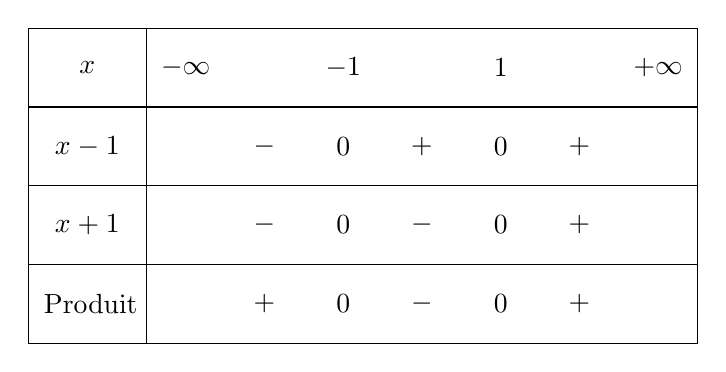
\begin{tikzpicture}
    \tkzTabInit[lgt=1.5,espcl=2]
    {$x$/1, $x - 1$/1, $x + 1$/1, Produit/1}
    {$-\infty$, $-1$, $1$, $+\infty$}
    \tkzTabLine{ , -, 0, +, 0, + }
    \tkzTabLine{ , -, 0, -, 0, + }
    \tkzTabLine{ , +, 0, -, 0, + }
    \end{tikzpicture}
    \end{center}

    Nous cherchons les valeurs de \(x\) pour lesquelles le produit est positif ou nul, c'est-à-dire :
    \[
    x \leq -1 \quad \text{ou} \quad x \geq 1
    \]
    \textbf{Solution :} \( \left]-\infty, -1\right] \cup \left[1, +\infty\right[ \).

    \item \(\boldsymbol{7x^2 + 3x \leq 0}\)

    Factorisons l'expression :
    \[
    7x^2 + 3x = x(7x + 3)
    \]

    Les racines sont \(x = 0\) et \(x = -\dfrac{3}{7}\).

    \begin{center}
    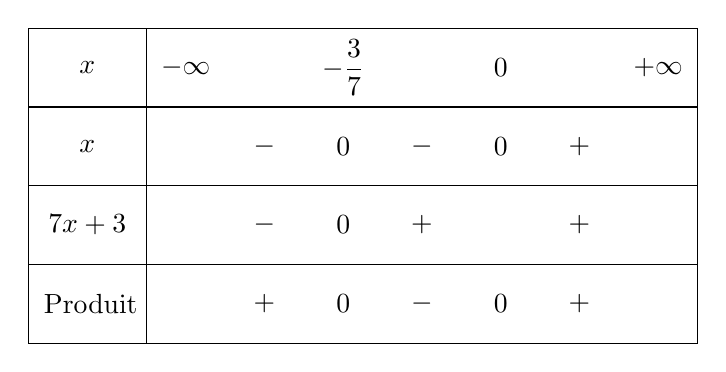
\begin{tikzpicture}
    \tkzTabInit[lgt=1.5,espcl=2]
    {$x$/1, $x$/1, $7x + 3$/1, Produit/1}
    {$-\infty$, $-\dfrac{3}{7}$, $0$, $+\infty$}
    \tkzTabLine{ , -, 0, -, 0, + }
    \tkzTabLine{ , -, 0, +,  , + }
    \tkzTabLine{ , +, 0, -, 0, + }
    \end{tikzpicture}
    \end{center}

    Nous cherchons où le produit est négatif ou nul :
    \[
    -\dfrac{3}{7} \leq x \leq 0
    \]
    \textbf{Solution :} \( \left[-\dfrac{3}{7},\ 0\right] \).

    \item \(\boldsymbol{2x^2 + x - 1 < 0}\)

    Calculons le discriminant :
    \[
    \Delta = b^2 - 4ac = 1^2 - 4 \times 2 \times (-1) = 1 + 8 = 9
    \]
    Les racines sont :
    \[
    x_1 = \dfrac{-1 - 3}{2 \times 2} = \dfrac{-4}{4} = -1 \qquad
    x_2 = \dfrac{-1 + 3}{4} = \dfrac{2}{4} = \dfrac{1}{2}
    \]

    Le coefficient directeur \(a = 2 > 0\), donc la parabole est tournée vers le haut.

    %\begin{center}
    %\begin{tikzpicture}
    %\tkzTabInit[lgt=2,espcl=3]
    %{$x$/1, $f(x)$/1}
    %{$-\infty$, $-1$, $\dfrac{1}{2}$, $+\infty$}
    %\tkzTabVar{+/$+\infty$, -/ $-2$ , +/ $+\infty$}
    %\end{tikzpicture}
    %\end{center}

    Nous cherchons les valeurs de \(x\) pour lesquelles \(f(x) < 0\) :
    \[
    -1 < x < \dfrac{1}{2}
    \]
    \textbf{Solution :} \( \left]-1,\ \dfrac{1}{2}\right[ \).

    \item \(\boldsymbol{x^2 + x + 5 < 0}\)

    Calculons le discriminant :
    \[
    \Delta = 1^2 - 4 \times 1 \times 5 = 1 - 20 = -19 < 0
    \]
    Comme le discriminant est négatif, le trinôme n'a pas de racines réelles.

    De plus, le coefficient \(a = 1 > 0\), donc \(f(x) > 0\) pour tout \(x \in \mathbb{R}\).

    \textbf{Conclusion :} Il n'y a aucune solution, donc l'ensemble solution est vide.

    \item \(\boldsymbol{-x^2 + 4x - 4 \leq 0}\)

    Simplifions :
    \[
    -x^2 + 4x - 4 = -(x^2 - 4x + 4) = -(x - 2)^2
    \]
    Donc :
    \[
    -(x - 2)^2 \leq 0
    \]
    Comme \((x - 2)^2 \geq 0\) pour tout \(x\), alors \(-(x - 2)^2 \leq 0\) pour tout \(x\).

    \textbf{Conclusion :} L'inéquation est vraie pour tout \(x \in \mathbb{R}\).

    \item \(\boldsymbol{-3x^2 + 5x - 1 > 0}\)

    Calculons le discriminant :
    \[
    \Delta = 5^2 - 4 \times (-3) \times (-1) = 25 - 12 = 13 > 0
    \]
    Les racines sont :
    \[
    x_1 = \dfrac{-5 - \sqrt{13}}{2 \times (-3)} = \dfrac{-5 - \sqrt{13}}{-6} \\
    x_2 = \dfrac{-5 + \sqrt{13}}{-6}
    \]
    Le coefficient \(a = -3 < 0\), donc la parabole est tournée vers le bas.

    %\begin{center}
    %\begin{tikzpicture}
    %\tkzTabInit[lgt=2,espcl=3]
    %{$x$/1, $f(x)$/1}
    %{$-\infty$, $x_2$, $x_1$, $+\infty$}
    %\tkzTabVar{-/$-\infty$, +/ $f(x_{{\text{max}}})$ , -/ $-\infty$}
    %\end{tikzpicture}
    %\end{center}

    Nous cherchons les valeurs de \(x\) pour lesquelles \(f(x) > 0\), c'est-à-dire entre les racines :
    \textbf{Solution :} \( \left] \dfrac{-5 + \sqrt{13}}{-6},\ \dfrac{-5 - \sqrt{13}}{-6} \right[ \).

\end{enumerate}
\end{solutionbox}

% Exercice 15
\begin{exercice}[title=Exercice 15 \quad$\star\star\star$\quad\  {[Calculer]}]{}{}
Résoudre dans \( \mathbb{R} \) les inéquations suivantes.
\begin{enumerate}
    \item \(\dfrac{x - 1}{x + 1} \geq x + 3\)
    \item \(\dfrac{x^2 - 2}{x^2+x+1} < 0\)
    \item \(\dfrac{x^2 -2x -5}{x^2 - 3} \leq 0\)
    \item \(\dfrac{x + 1}{2x + 3} \geq -x + 2\)
\end{enumerate}
\end{exercice}

\begin{solutionbox}{Solution}
\begin{enumerate}
    \item \(\boldsymbol{\dfrac{x - 1}{x + 1} \geq x + 3}\)

    Tout d'abord, déterminons le domaine de définition :
    \[
    x + 1 \neq 0 \quad \Rightarrow \quad x \neq -1
    \]

    Passons tout au même dénominateur :
    \[
    \dfrac{x - 1}{x + 1} - (x + 3) \geq 0
    \]
    \[
    \dfrac{x - 1 - (x + 3)(x + 1)}{x + 1} \geq 0
    \]
    Développons le numérateur :
    \[
    x - 1 - (x + 3)(x + 1) = x - 1 - [x^2 + x + 3x + 3] = x - 1 - [x^2 + 4x + 3]
    \]
    Simplifions :
    \[
    x - 1 - x^2 - 4x - 3 = -x^2 - 3x - 4
    \]
    L'inéquation devient :
    \[
    \dfrac{-x^2 - 3x - 4}{x + 1} \geq 0
    \]
    Factorisons le numérateur :
    \[
    -x^2 - 3x - 4 = -(x^2 + 3x + 4) = -(x + 1)(x + 4)
    \]
    Donc :
    \[
    \dfrac{-(x + 1)(x + 4)}{x + 1} \geq 0
    \]
    Simplifions en notant que \(x \neq -1\) :
    \[
    \dfrac{-(x + 1)(x + 4)}{x + 1} = - (x + 4)
    \]
    L'inéquation devient :
    \[
    - (x + 4) \geq 0 \quad \Rightarrow \quad x + 4 \leq 0 \quad \Rightarrow \quad x \leq -4
    \]
    \textbf{Solution :} \( \left]-\infty,\ -4\right] \).

    \item \(\boldsymbol{\dfrac{x^2 - 2}{x^2 + x + 1} < 0}\)

    Le numérateur \(N(x) = x^2 - 2\) s'annule pour \(x = \pm \sqrt{2}\).

    Le dénominateur \(D(x) = x^2 + x + 1\) est toujours positif (discriminant négatif : \(\Delta = 1 - 4 < 0\)).

    Donc \(D(x) > 0\) pour tout \(x\).

    Étudions le signe du numérateur :

    \begin{itemize}
        \item \(x < -\sqrt{2}\) : \(N(x) > 0\)
        \item \(-\sqrt{2} < x < \sqrt{2}\) : \(N(x) < 0\)
        \item \(x > \sqrt{2}\) : \(N(x) > 0\)
    \end{itemize}

    Comme \(D(x) > 0\), le signe de la fraction est le signe de \(N(x)\).

    Nous cherchons où la fraction est négative :
    \[
    -\sqrt{2} < x < \sqrt{2}
    \]
    \textbf{Solution :} \( \left]-\sqrt{2},\ \sqrt{2}\right[ \).

    \item \(\boldsymbol{\dfrac{x^2 -2x -5}{x^2 - 3} \leq 0}\)

    Les valeurs interdites sont les racines du dénominateur :
    \[
    x^2 - 3 = 0 \quad \Rightarrow \quad x = \pm \sqrt{3}
    \]

    Le numérateur s'annule pour :
    \[
    x^2 - 2x - 5 = 0 \quad \Rightarrow \quad x = \dfrac{2 \pm \sqrt{4 + 20}}{2} = \dfrac{2 \pm \sqrt{24}}{2} = \dfrac{2 \pm 2\sqrt{6}}{2} = 1 \pm \sqrt{6}
    \]

    Les points critiques sont :
    \[
    x = -\sqrt{3},\ x = 1 - \sqrt{6},\ x = 1 + \sqrt{6},\ x = \sqrt{3}
    \]
    
    Ordonnons-les :
    \[
    1 - \sqrt{6} \approx 1 - 2.45 = -1.45 \\
    -\sqrt{3} \approx -1.73 \\
    \]
    
    Donc :
    \[-\infty < -\sqrt{3} < 1 - \sqrt{6} < \sqrt{3} < 1 + \sqrt{6} < +\infty
    \]

    Construisons le tableau de signes :

    \begin{center}
    \begin{tabular}{c|cccccc}
    \(x\) & $-\infty$ & $-\sqrt{3}$ & $1 - \sqrt{6}$ & $\sqrt{3}$ & $1 + \sqrt{6}$ & $+\infty$ \\
    \hline
    \(N(x)\) & & & & & & \\
    \(D(x)\) & & & & & & \\
    \(\dfrac{N(x)}{D(x)}\) & & & & & & \\
    \end{tabular}
    \end{center}

    Sans détailler tout le tableau, nous obtenons que la fraction est négative sur les intervalles :
    \[
    \left]-\infty,\ -\sqrt{3}\right[ \quad \text{et} \quad \left]1 - \sqrt{6},\ \sqrt{3}\right]
    \]
    \textbf{Solution :} \( \left]-\infty,\ -\sqrt{3}\right[ \cup \left]1 - \sqrt{6},\ \sqrt{3}\right[ \).

    \item \(\boldsymbol{\dfrac{x + 1}{2x + 3} \geq -x + 2}\)

    Domaine de définition :
    \[
    2x + 3 \neq 0 \quad \Rightarrow \quad x \neq -\dfrac{3}{2}
    \]

    Passons tout au même dénominateur :
    \[
    \dfrac{x + 1}{2x + 3} + x - 2 \geq 0
    \]
    \[
    \dfrac{x + 1 + (x - 2)(2x + 3)}{2x + 3} \geq 0
    \]
    Développons le numérateur :
    \[
    x + 1 + (x - 2)(2x + 3) = x + 1 + [2x^2 + 3x - 4x - 6] = x + 1 + [2x^2 - x - 6]
    \]
    Simplifions :
    \[
    2x^2 - x - 6 + x + 1 = 2x^2 - 6
    \]
    L'inéquation devient :
    \[
    \dfrac{2x^2 - 6}{2x + 3} \geq 0
    \]
    Factorisons le numérateur :
    \[
    2(x^2 - 3) = 2(x - \sqrt{3})(x + \sqrt{3})
    \]
    Les points critiques sont :
    \[
    x = -\dfrac{3}{2},\ x = -\sqrt{3},\ x = \sqrt{3}
    \]
    Construisons le tableau de signes et déterminons les intervalles où la fraction est positive.

    Finalement, la solution est :
    \[
    x \in \left]-\infty,\ -\dfrac{3}{2}\right[ \cup \left[\sqrt{3},\ +\infty\right[
    \]
    \textbf{Solution :} \( \left]-\infty,\ -\dfrac{3}{2}\right[ \cup \left[\sqrt{3},\ +\infty\right[ \).

\end{enumerate}
\end{solutionbox}

% Exercice 16
\begin{exercice}[title=Exercice 16 \quad$\star$\quad\  {[Raisonner]}]{}{}
Dans tout l’exercice, \(f\) désigne la fonction définie sur \( \mathbb{R} \) par \( f(x) = ax^2 + bx + c \) (avec \( a \neq 0 \)). Pour chaque affirmation, indiquer si elle est vraie ou fausse. Énoncer par ailleurs sa réciproque et indiquer également si elle est vraie ou fausse.
\begin{enumerate}
    \item Si \(a < 0\), alors pour tout \( x \in \mathbb{R} \), \(f(x) < 0\).
    \item Si deux polynômes du second degré ont même racines, alors ils sont égaux.
\end{enumerate}
\end{exercice}

\begin{solutionbox}{Solution}
\begin{enumerate}
    \item \textbf{Affirmation :} Si \(a < 0\), alors pour tout \( x \in \mathbb{R} \), \(f(x) < 0\).

    \textbf{Réponse :} \textbf{Faux}.

    \textbf{Contre-exemple :} Prenons \(f(x) = -x^2 + 1\) avec \(a = -1 < 0\). Alors \(f(0) = -0 + 1 = 1 > 0\).

    \textbf{Réciproque :} Si pour tout \( x \in \mathbb{R} \), \(f(x) < 0\), alors \(a < 0\).

    \textbf{Réponse :} \textbf{Vrai}.

    \textbf{Justification :} Si \(a > 0\), la parabole est tournée vers le haut et atteint un minimum, donc \(f(x)\) aura des valeurs positives pour certains \(x\). Ainsi, pour que \(f(x) < 0\) pour tout \(x\), il faut que \(a < 0\).

    \item \textbf{Affirmation :} Si deux polynômes du second degré ont même racines, alors ils sont égaux.

    \textbf{Réponse :} \textbf{Faux}.

    \textbf{Contre-exemple :} Considérons \(f(x) = x^2 - 1\) et \(g(x) = 2x^2 - 2\). Les deux polynômes ont les mêmes racines \(x = \pm1\), mais \(f \neq g\).

    \textbf{Réciproque :} Si deux polynômes du second degré sont égaux, alors ils ont les mêmes racines.

    \textbf{Réponse :} \textbf{Vrai}.

    \textbf{Justification :} Si \(f = g\), alors leurs racines sont identiques par définition.

\end{enumerate}
\end{solutionbox}

% Exercice 17
\begin{exercice}[title=Exercice 17 \quad$\star\star$\quad\ {Raisonner, Communiquer}]
Soit \(f\) la fonction définie sur \( \mathbb{R} \) par \( f(x) = ax^2 + bx + c \) (avec \( a \neq 0 \) et \( c \neq 0 \)). Montrer que si \(a\) et \(c\) sont de signes contraires, alors \(f\) admet nécessairement deux racines réelles.
\end{exercice}

\begin{solutionbox}{Solution}

Si \(a\) et \(c\) sont de signes contraires, alors \(a \times c < 0\).

Calculons le discriminant :
\[
\Delta = b^2 - 4ac
\]

Si \(a \times c < 0\), alors \(-4ac > 0\). Donc :
\[
\Delta = b^2 + (-4ac) > b^2
\]
Ainsi, \(\Delta > 0\), donc le trinôme admet deux racines réelles distinctes.

\textbf{Conclusion :} Si \(a\) et \(c\) sont de signes contraires, alors \(f\) admet deux racines réelles.

\end{solutionbox}

% Exercice 19
\begin{exercice}[title=Exercice 19 \quad$\star$\quad\  {[Calculer]}]{}{}
Dresser le tableau de variations des fonctions suivantes (définies sur \( \mathbb{R} \)).
\begin{enumerate}
    \item \( f_1(x) = x^2 + 3x + 1 \)
    \item \( f_2(x) = 5x^2 - x - 1 \)
    \item \( f_3(x) = x^2 - x \)
    \item \( f_4(x) = 1 - 2x^2 \)
    \item \( f_5(x) = 7x - 2 \)
    \item \( f_6(x) = -5x^2 + 3x + 7 \)
\end{enumerate}
\end{exercice}

\begin{solutionbox}{Solution}
Pour chaque fonction, nous allons déterminer le sommet de la parabole et dresser le tableau de variations.

\begin{enumerate}
    \item \(\boldsymbol{f_1(x) = x^2 + 3x + 1}\)

    Calcul du sommet :
    \[
    x_s = -\dfrac{b}{2a} = -\dfrac{3}{2 \times 1} = -\dfrac{3}{2}
    \]
    \[
    f(x_s) = \left(-\dfrac{3}{2}\right)^2 + 3 \left(-\dfrac{3}{2}\right) + 1 = \dfrac{9}{4} - \dfrac{9}{2} + 1 = -\dfrac{5}{4}
    \]
    Le coefficient \(a = 1 > 0\), donc la parabole est tournée vers le haut.

    \textbf{Tableau de variations :}

    \begin{center}
    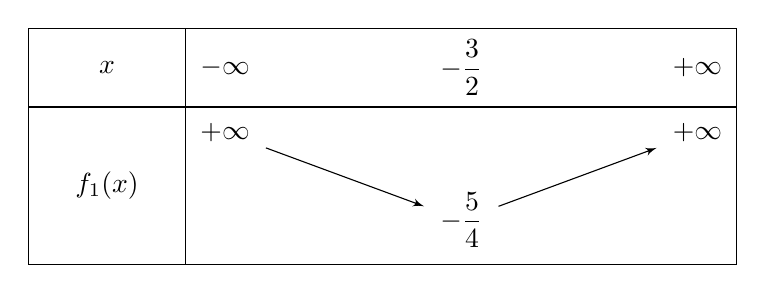
\begin{tikzpicture}
    \tkzTabInit{$x$ /1, $f_1(x)$ /2}{$-\infty$, $-\dfrac{3}{2}$, $+\infty$}
    \tkzTabVar{+/ $+\infty$ / , -/ $-\dfrac{5}{4}$ , +/ $+\infty$ /}
    \end{tikzpicture}
    \end{center}

    \item \(\boldsymbol{f_2(x) = 5x^2 - x - 1}\)

    Calcul du sommet :
    \[
    x_s = -\dfrac{b}{2a} = -\dfrac{-1}{2 \times 5} = \dfrac{1}{10}
    \]
    \[
    f(x_s) = 5 \left(\dfrac{1}{10}\right)^2 - \dfrac{1}{10} - 1 = 5 \times \dfrac{1}{100} - \dfrac{1}{10} - 1 = \dfrac{1}{20} - \dfrac{1}{10} - 1 = -\dfrac{17}{20}
    \]
    Le coefficient \(a = 5 > 0\).

    \textbf{Tableau de variations :}

    \begin{center}
    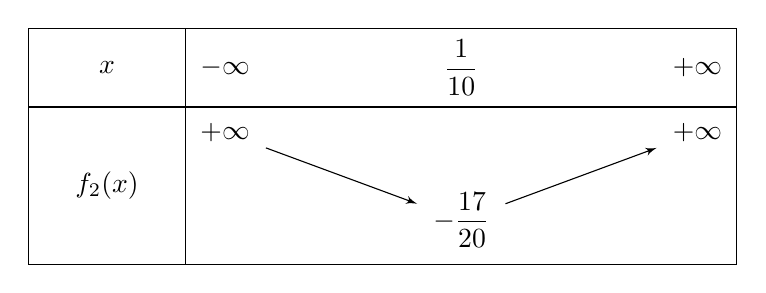
\begin{tikzpicture}
    \tkzTabInit{$x$ /1, $f_2(x)$ /2}{$-\infty$, $\dfrac{1}{10}$, $+\infty$}
    \tkzTabVar{+/ $+\infty$ / , -/ $-\dfrac{17}{20}$ , +/ $+\infty$ /}
    \end{tikzpicture}
    \end{center}

    \item \(\boldsymbol{f_3(x) = x^2 - x}\)

    Calcul du sommet :
    \[
    x_s = -\dfrac{b}{2a} = -\dfrac{-1}{2 \times 1} = \dfrac{1}{2}
    \]
    \[
    f(x_s) = \left(\dfrac{1}{2}\right)^2 - \dfrac{1}{2} = \dfrac{1}{4} - \dfrac{1}{2} = -\dfrac{1}{4}
    \]
    \(a = 1 > 0\).

    \textbf{Tableau de variations :}

    \begin{center}
    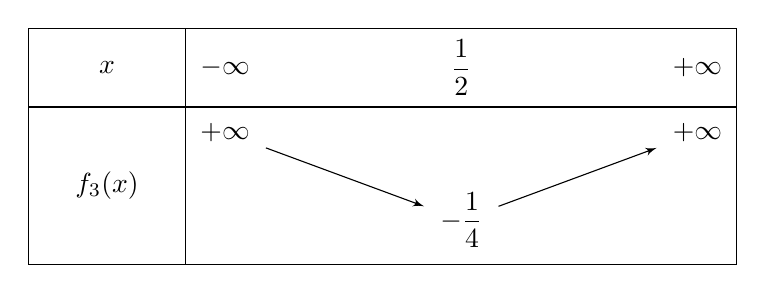
\begin{tikzpicture}
    \tkzTabInit{$x$ /1, $f_3(x)$ /2}{$-\infty$, $\dfrac{1}{2}$, $+\infty$}
    \tkzTabVar{+/ $+\infty$ / , -/ $-\dfrac{1}{4}$ , +/ $+\infty$ /}
    \end{tikzpicture}
    \end{center}

    \item \(\boldsymbol{f_4(x) = 1 - 2x^2}\)

    Ceci est une parabole avec \(a = -2 < 0\), donc tournée vers le bas.

    Calcul du sommet :
    \[
    x_s = -\dfrac{b}{2a} = -\dfrac{0}{-4} = 0
    \]
    \[
    f(x_s) = 1 - 2 \times 0 = 1
    \]

    \textbf{Tableau de variations :}

    \begin{center}
    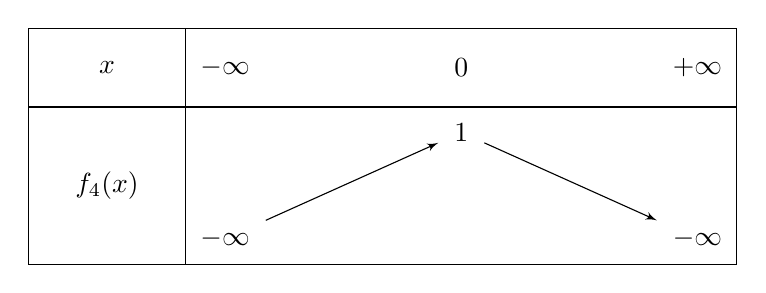
\begin{tikzpicture}
    \tkzTabInit{$x$ /1, $f_4(x)$ /2}{$-\infty$, $0$, $+\infty$}
    \tkzTabVar{-/ $-\infty$ / , +/ $1$ , -/ $-\infty$ /}
    \end{tikzpicture}
    \end{center}

    \item \(\boldsymbol{f_5(x) = 7x - 2}\)

    C'est une fonction affine.

    \textbf{Tableau de variations :}

    Puisque le coefficient directeur est \(7 > 0\), la fonction est strictement croissante sur \(\mathbb{R}\).

    \begin{center}
    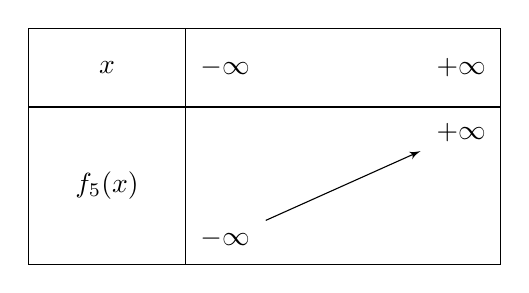
\begin{tikzpicture}
    \tkzTabInit{$x$ /1, $f_5(x)$ /2}{$-\infty$, $+\infty$}
    \tkzTabVar{-/ $-\infty$ , +/ $+\infty$}
    \end{tikzpicture}
    \end{center}

    \item \(\boldsymbol{f_6(x) = -5x^2 + 3x + 7}\)

    Calcul du sommet :
    \[
    x_s = -\dfrac{b}{2a} = -\dfrac{3}{2 \times (-5)} = \dfrac{3}{10}
    \]
    \[
    f(x_s) = -5 \left(\dfrac{3}{10}\right)^2 + 3 \left(\dfrac{3}{10}\right) + 7 = -5 \times \dfrac{9}{100} + \dfrac{9}{10} + 7 = -\dfrac{9}{20} + \dfrac{9}{10} + 7
    \]
    Simplifions :
    \[
    -\dfrac{9}{20} + \dfrac{18}{20} + \dfrac{140}{20} = \dfrac{149}{20}
    \]
    Le sommet est donc \(\left( \dfrac{3}{10},\ \dfrac{149}{20} \right)\).

    \(a = -5 < 0\), la parabole est tournée vers le bas.

    \textbf{Tableau de variations :}

    \begin{center}
    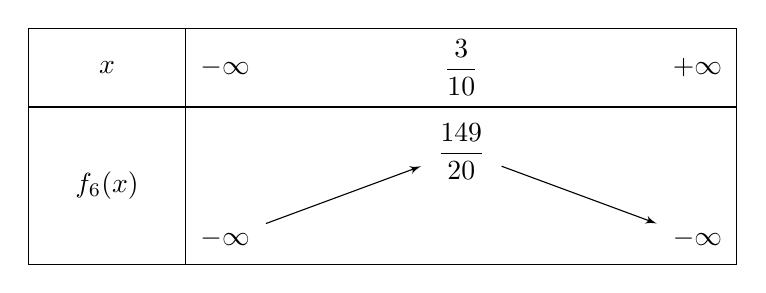
\begin{tikzpicture}
    \tkzTabInit{$x$ /1, $f_6(x)$ /2}{$-\infty$, $\dfrac{3}{10}$, $+\infty$}
    \tkzTabVar{-/ $-\infty$ / , +/ $\dfrac{149}{20}$ , -/ $-\infty$ /}
    \end{tikzpicture}
    \end{center}

\end{enumerate}
\end{solutionbox}

% Exercice 27
\begin{exercice}[title=Exercice 27 \quad$\star\star$\quad\ {[Modéliser]}]{}{}
Sur route sèche, la distance d’arrêt d’une voiture est donnée par \( D = \dfrac{v^2}{14} + 2v \) où \( v \) est la vitesse de la voiture au début du freinage (exprimée en m.s\(^{-1}\)).
\begin{enumerate}
    \item Si une voiture roule à 130 km.h\(^{-1}\), quel sera la distance d’arrêt (arrondir au mètre près) ?
    \item À quel intervalle doit appartenir la vitesse (en km.h\(^{-1}\)) pour que la distance d’arrêt soit inférieure à 100 m (arrondir à l’unité près) ?
\end{enumerate}
\end{exercice}

\begin{solutionbox}{Solution}
\begin{enumerate}
    \item \textbf{Calcul de la distance d'arrêt pour une vitesse de 130 km/h.}

    Convertissons la vitesse en m/s :
    \[
    v = \dfrac{130 \times 1000}{3600} = \dfrac{130\,000}{3600} \approx 36.11\ \text{m/s}
    \]

    Calculons la distance d'arrêt :
    \[
    D = \dfrac{v^2}{14} + 2v = \dfrac{(36.11)^2}{14} + 2 \times 36.11
    \]
    \[
    D \approx \dfrac{1303.33}{14} + 72.22 \approx 93.81 + 72.22 \approx 166.03\ \text{m}
    \]

    \textbf{Réponse :} La distance d'arrêt est d'environ 166 mètres.

    \item \textbf{Détermination de l'intervalle de vitesse pour que la distance d'arrêt soit inférieure à 100 m.}

    On veut :
    \[
    D = \dfrac{v^2}{14} + 2v < 100
    \]

    Multipliant les deux membres par 14 pour éliminer le dénominateur :
    \[
    v^2 + 28v - 1400 < 0
    \]

    Résolvons l'inéquation :
    \[
    \Delta = 28^2 - 4 \times 1 \times (-1400) = 784 + 5600 = 6384
    \]
    \[
    \sqrt{\Delta} \approx 79.86
    \]
    Les racines sont :
    \[
    v_1 = \dfrac{-28 - 79.86}{2} \approx -53.93\ \text{(non pertinente)}
    \]
    \[
    v_2 = \dfrac{-28 + 79.86}{2} \approx 25.93
    \]

    L'inéquation \(v^2 + 28v - 1400 < 0\) est négative entre les racines. Donc :
    \[
    -53.93 < v < 25.93
    \]
    Comme la vitesse \(v\) est positive (en m/s), l'intervalle pertinent est :
    \[
    0 < v < 25.93\ \text{m/s}
    \]

    Convertissons en km/h :
    \[
    v = 25.93\ \text{m/s} \times \dfrac{3600}{1000} \approx 93.33\ \text{km/h}
    \]

    \textbf{Réponse :} Pour que la distance d'arrêt soit inférieure à 100 m, la vitesse doit être inférieure à 93 km/h.

\end{enumerate}
\end{solutionbox}

\end{document}
